%%%%%%%%%%%%%%%%%%%%%%%%%%%%%%%%%%%%%%%%%
% Barbara Liskov Presentation
% LaTeX Template
% 23/11/2020
% 
%%%%%%%%%%%%%%%%%%%%%%%%%%%%%%%%%%%%%%%%%

%----------------------------------------------------------------------------------------
%	PACKAGES AND THEMES
%----------------------------------------------------------------------------------------

\documentclass{beamer}

\mode<presentation> {

\usetheme{Madrid}

}
\hypersetup{
    colorlinks=true,
    linkcolor=blue,
    filecolor=magenta,      
    urlcolor=cyan,
}
\usepackage{graphicx} 
\usepackage{booktabs} 
\usepackage{hyperref} 
\usepackage{listings}

\usepackage{xcolor}

\definecolor{codegreen}{rgb}{0,0.6,0}
\definecolor{codegray}{rgb}{0.5,0.5,0.5}
\definecolor{codepurple}{rgb}{0.58,0,0.82}
\definecolor{backcolour}{rgb}{0.95,0.95,0.92}



\lstdefinestyle{mystyle}{
    backgroundcolor=\color{backcolour},   
    commentstyle=\color{codegreen},
    keywordstyle=\color{magenta},
    numberstyle=\tiny\color{codegray},
    stringstyle=\color{codepurple},
    basicstyle=\ttfamily\footnotesize,
    breakatwhitespace=false,         
    breaklines=true,                 
    captionpos=b,                    
    keepspaces=true,                 
    numbers=left,                    
    numbersep=5pt,                  
    showspaces=false,                
    showstringspaces=false,
    showtabs=false,                  
    tabsize=2
}

\lstset{style=mystyle}
%----------------------------------------------------------------------------------------
%	TITLE PAGE
%----------------------------------------------------------------------------------------

\title[Research Methods]{Barbara Liskov}
\author{Group N}
\institute[GMIT]
{
\textit{Grace Keane} \\\textit{Shirin Nagle} \\ 
\medskip
}
\date{}

\begin{document}

\begin{frame}
\titlepage % Print the title page as the first slide
\end{frame}

%----------------------------------------------------------------------------------------
%	BRIEF DESCRIPTION
%----------------------------------------------------------------------------------------

\begin{frame}
\frametitle{Brief Description} 

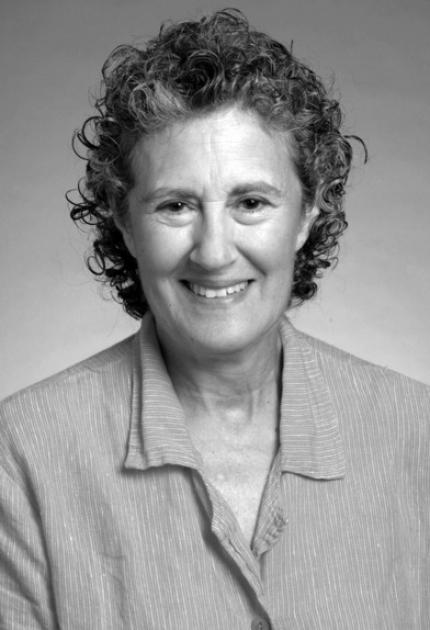
\includegraphics[scale=0.4, align=centre]{Barbara Liskov}
\centering

\end{frame}


%----------------------------------------------------------------
%	PRESENTATION SLIDES
%----------------------------------------------------------------


%------------------------------------------------


\begin{frame}
\frametitle{Important Details}
\begin{itemize}
\item Computer Scientist
\item Born: November 7th, 1939, California
\item One of the first women in the USA to be awarded a PhD in Computer Science
\item She is one of the world's leading authorities on computer language and system design
\item She won numerous awards as well as the Turing award in 2009
\item Since 1966, 70 computer scientists have won the Turing Award. Only 3 have been women. Therefore this is an amazing achievement
\item Created the Liskov's substitution principle
\end{itemize}
\end{frame}

%------------------------------------------------

\begin{frame}
\frametitle{Turing Award}
Barbara Liskov was awarded the Alan Turing award for  contributions "of lasting and major technical importance to the computer field". 

\vspace{5mm} %5mm vertical space

Her award was for contributions to practical and theoretical foundations of programming language and system design, especially related to data abstraction, fault tolerance, and distributed computing. 

\vspace{5mm}

She developed a new notion of sub typing known as the Liskov Substitution principle.

\vspace{5mm} %5mm vertical space

At a high level, the LSP states that in an object-oriented program, if we substitute a superclass object reference with an object of any of its subclasses, the program should not break.\\

\vspace{1mm}

\href{https://reflectoring.io/lsp-explained/}{click reflectoring website}
\end{frame}

%------------------------------------------------

\begin{frame}
\frametitle{Barbara Liskov's definition}
"If for each object o1 of type S there is an object o2 of type T such that for all programs P defined in terms of T, the behavior of P is unchanged when o1 is substituted for o2 then S is a subtype of T"
\end{frame}



%------------------------------------------------

\vspace{5mm}

% Putting code on screen & formatted nicely
\begin{lstlisting}[language=Java]

// Animal super class 
public static class Animal {
  public String favoriteFood;
  public Animal(String favoriteFood) {
    this.favoriteFood = favoriteFood;
  }
}
// Subclass
public static class Dog extends Animal {
  public Dog(String favoriteFood) {
    super(favoriteFood);
  }
}

// Subclass
public static class Cat extends Animal {
  public Cat(String favoriteFood) {
    super(favoriteFood);
  }
}
\end{lstlisting}

\vspace{5mm}

%------------------------------------------------

%------------------------------------------------

\vspace{5mm}

% Putting code on screen & formatted nicely
\begin{lstlisting}[language=Java]
// Method to give treats
public static void GiveTreatTo(Animal animal) {
  String msg = "You fed the " + animal.getClass().getSimpleName() + " some "  + animal.favoriteFood;
  System.out.println(msg);
}

// Assigning treats to animals
// Do not have to create a new method per animal because of the LSP principle
public static void main(String[] args) {
  Dog rover = new Dog("bacon");
  Cat bingo = new Cat("fish");

  GiveTreatTo(rover);
  GiveTreatTo(bingo);
}


Command prompt output:

You gave the Dog some bacon
You gave the Cat some fish
\end{lstlisting}

%------------------------------------------------

\begin{frame}
\frametitle{SOLID} 


\includegraphics[scale=0.8, align=centre]{SOLID}
\centering

\end{frame}

%------------------------------------------------

\begin{frame}
\frametitle{Principle naming}
She did not name the Liskov Substitution Principle. Apparently, she received an email in the 90’s by somebody asking her whether he got her principle right, surprising her. She had not known that the principle had borne her name for years in the community.
\end{frame}

%------------------------------------------------

\begin{frame}
\Huge{\centerline{The End}}
\end{frame}

%----------------------------------------------------------------------------------------

\begin{frame}
\frametitle{Clickable References}
\begin{itemize}
\item \href{https://amturing.acm.org/award_winners/liskov_1108679.cfm}{ A.M. Turing; Barbara Liskov;} 

\item \href{https://reflectoring.io/lsp-explained/}{ Reflectoring; The Liskov Substitution Principle Explained;}

\item \href{https://www.geeksforgeeks.org/solid-principle-in-programming-understand-with-real-life-e}{GeeksforGeeks; SOLID Principle in Programming: Understand With Real Life Examples;}


\item \href{https://dev.to/erikwhiting88/liskov-substitution-principle-in-3-minutes-2}{DEV; Liskov Substitution Principle in 3 Minutes;}

\end{itemize}
\end{frame}

%-----------------------------------------------

\begin{frame}
\frametitle{GitHub link}

Organization used to manage our LaTeX presentation progression

\vspace{5mm}


\href{https://github.com/Research-Methods-Presentation}{GitHub organisation link} 

\end{frame}

%-----------------------------------------------

\begin{frame}
\Huge{\centerline{Questions?}}
\end{frame}

%-----------------------------------------------


\end{document} 